%%%%%%%%%%%%%%%%%%%%%%%%%%%%%%%%%%%%%%%%%%%%%%%%%%%%%%%%%%%%%%%%%%%%
%% chapter5.tex
%% UNL thesis document file
%%
%% Chapter with lots of dummy text
%%%%%%%%%%%%%%%%%%%%%%%%%%%%%%%%%%%%%%%%%%%%%%%%%%%%%%%%%%%%%%%%%%%%
\chapter{Research Plan}
\label{cha:plan}
\acresetall

\paragraph{Task I - Create a baseline using existing datasets for multimodal analysis.}
Given the existing datasets shown in chapter~\ref{cha:stateofart}, the RECOLA dataset will be used to create a baseline as it consists of video as well as physiological data which is labeled with emotions and facial expressions.
\todo{add second dataset}

\paragraph{Task IIa - Define a setup and experimental protocol and collect data from healthy and stuttering adults.}
Cooperation will be searched with the Stuttering Center of Pennsylvania which is located in Pittsburgh, to define the experimental protocol consulting a Speech and Language Therapist and to collect data from stutterers. Given the age group of the stutterers, voluntary subjects in the same age range will be recorded as control group.

\paragraph{Task IIb - Unimodal and multimodal analysis of the data collected from healthy subjects and stutterers.} Each modality will be analyzed separately as well as fused together. Hand-crafted features will be tested. The correlation of disfluencies detected through video and audio analysis and the emotional state measured through the EDA will be anaylzed.

\paragraph{Task IIc - Analyze influence of emotional biofeedback in stutter therapy over time.} Existing therapy exercises will be combined with emotional biofeedback. Given the insights from \textbf{Task 3}, the modalities which gather most information   will be used to collect data during several therapy sessions. As the collected data will represent the progress over time, a mathematical framework will be developed to represent the evolution over time.

\paragraph{Task IIIa - Define a setup and experimental protocol to collect data from subjects suffering dysarthria and apraxia of speech.} 
Cooperation will be searched with the Department of Neurology  from the University of Pittsburgh, to define the experimental protocol consulting a Speech and Language Therapist and to collect data from patients suffering dysarthria and apraxia of speech caused by an underlying neurodegenerative disease. 

\paragraph{Task IIIb - Unimodal and multimodal analysis of the data collected from subjects suffering dysarthria and apraxia of speech.}
Each modality will be analyzed separately as well as fused together. Hand-crafted features will be tested. The degree of emotional expressiveness detected through video and audio analysis and the emotional state measured through the EDA will be anaylzed.




\begin{figure}
\centering
\subbottom[]{
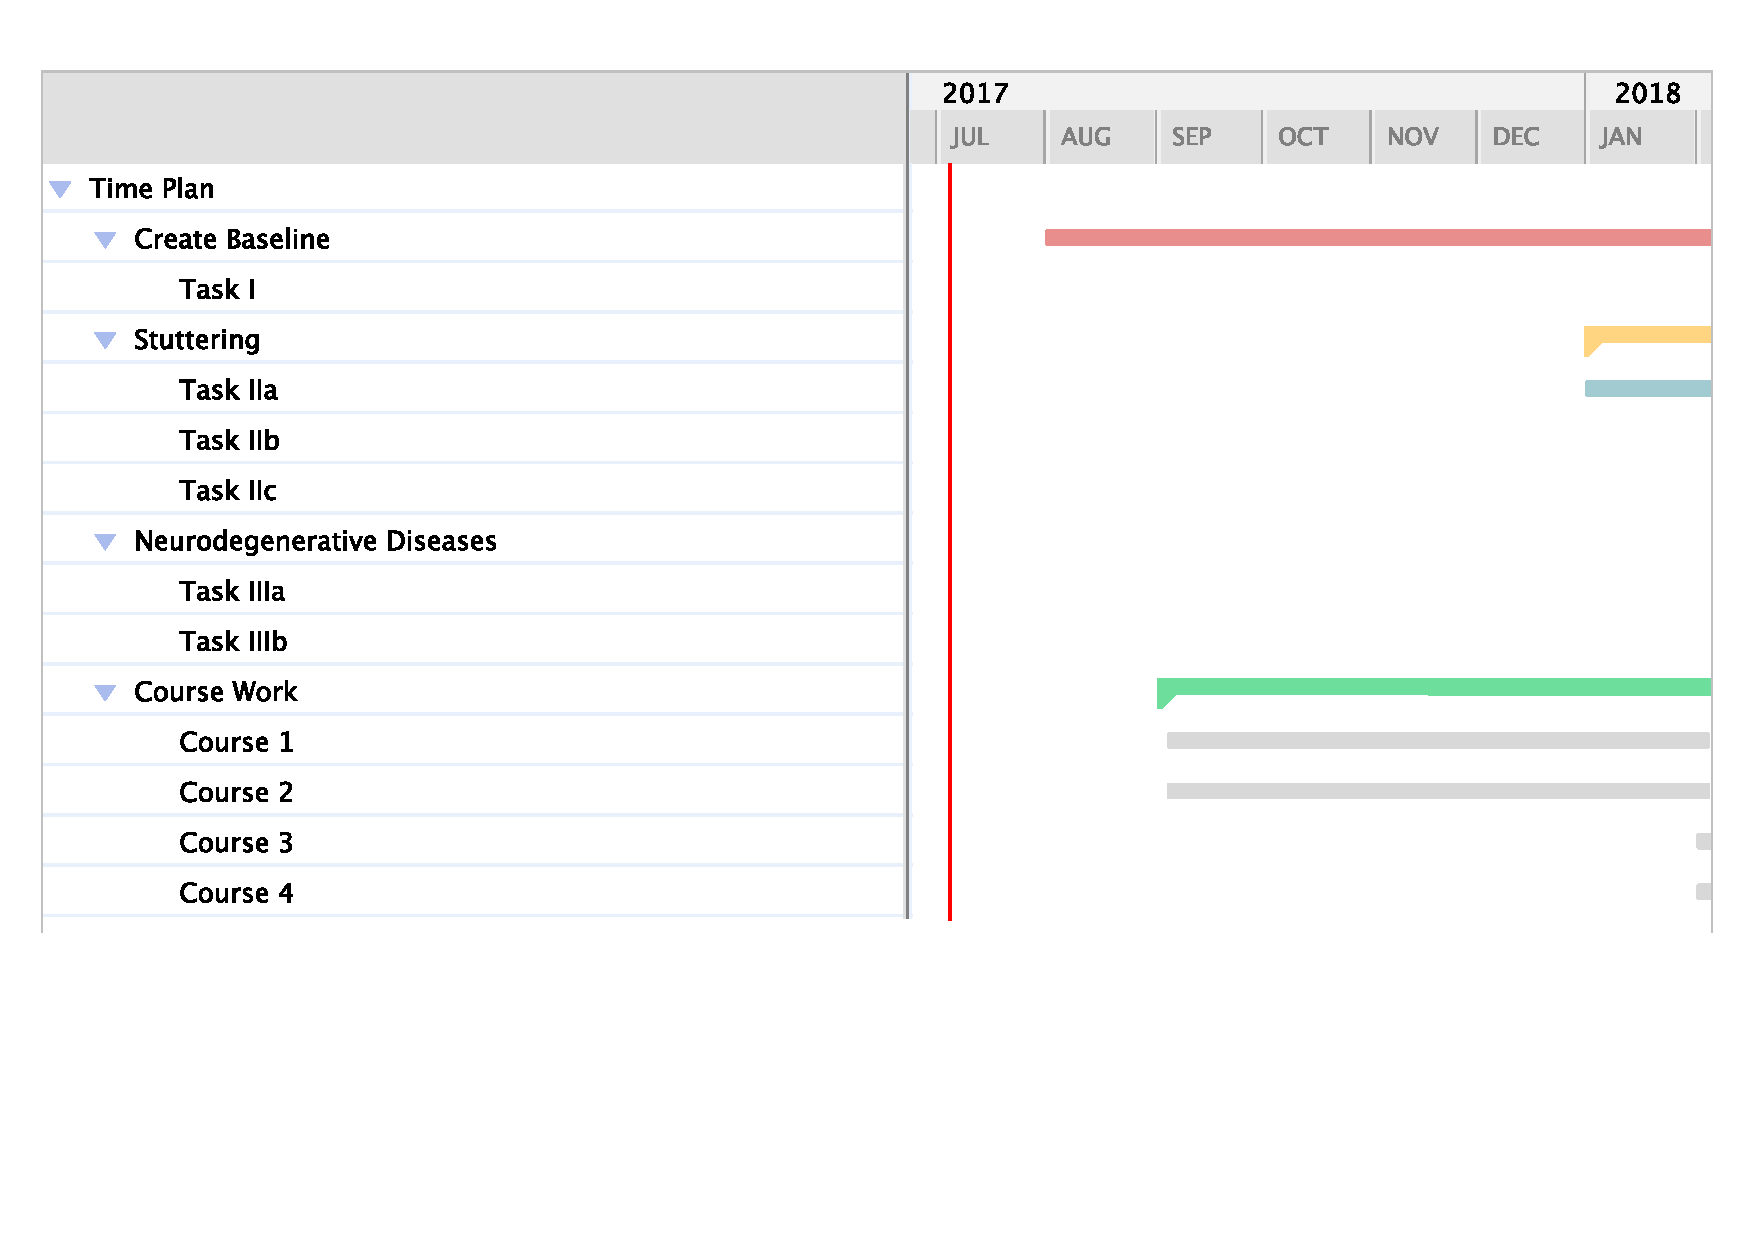
\includegraphics[width=13cm]{TimePlan1.pdf}}
\subbottom[]{
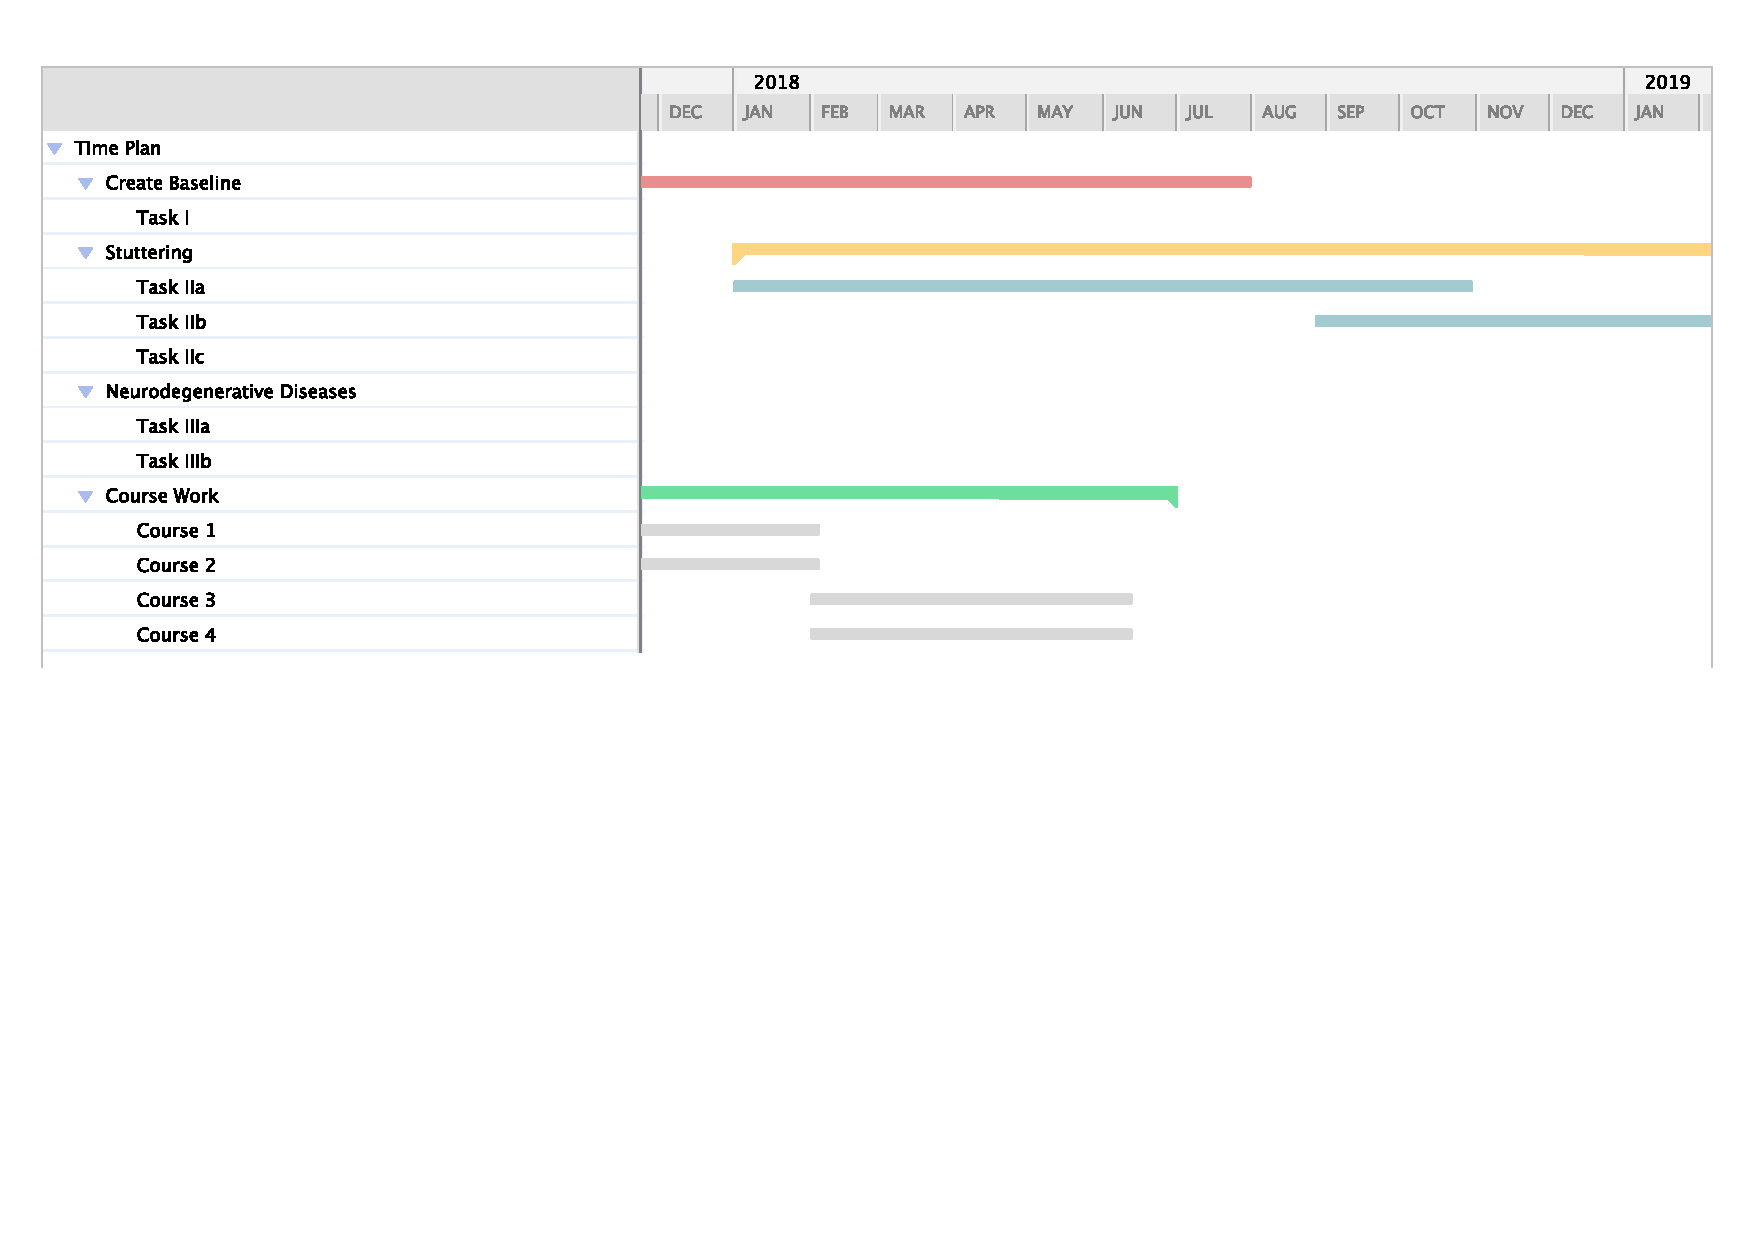
\includegraphics[width=15cm]{TimePlan2.pdf}}
\subbottom[]{
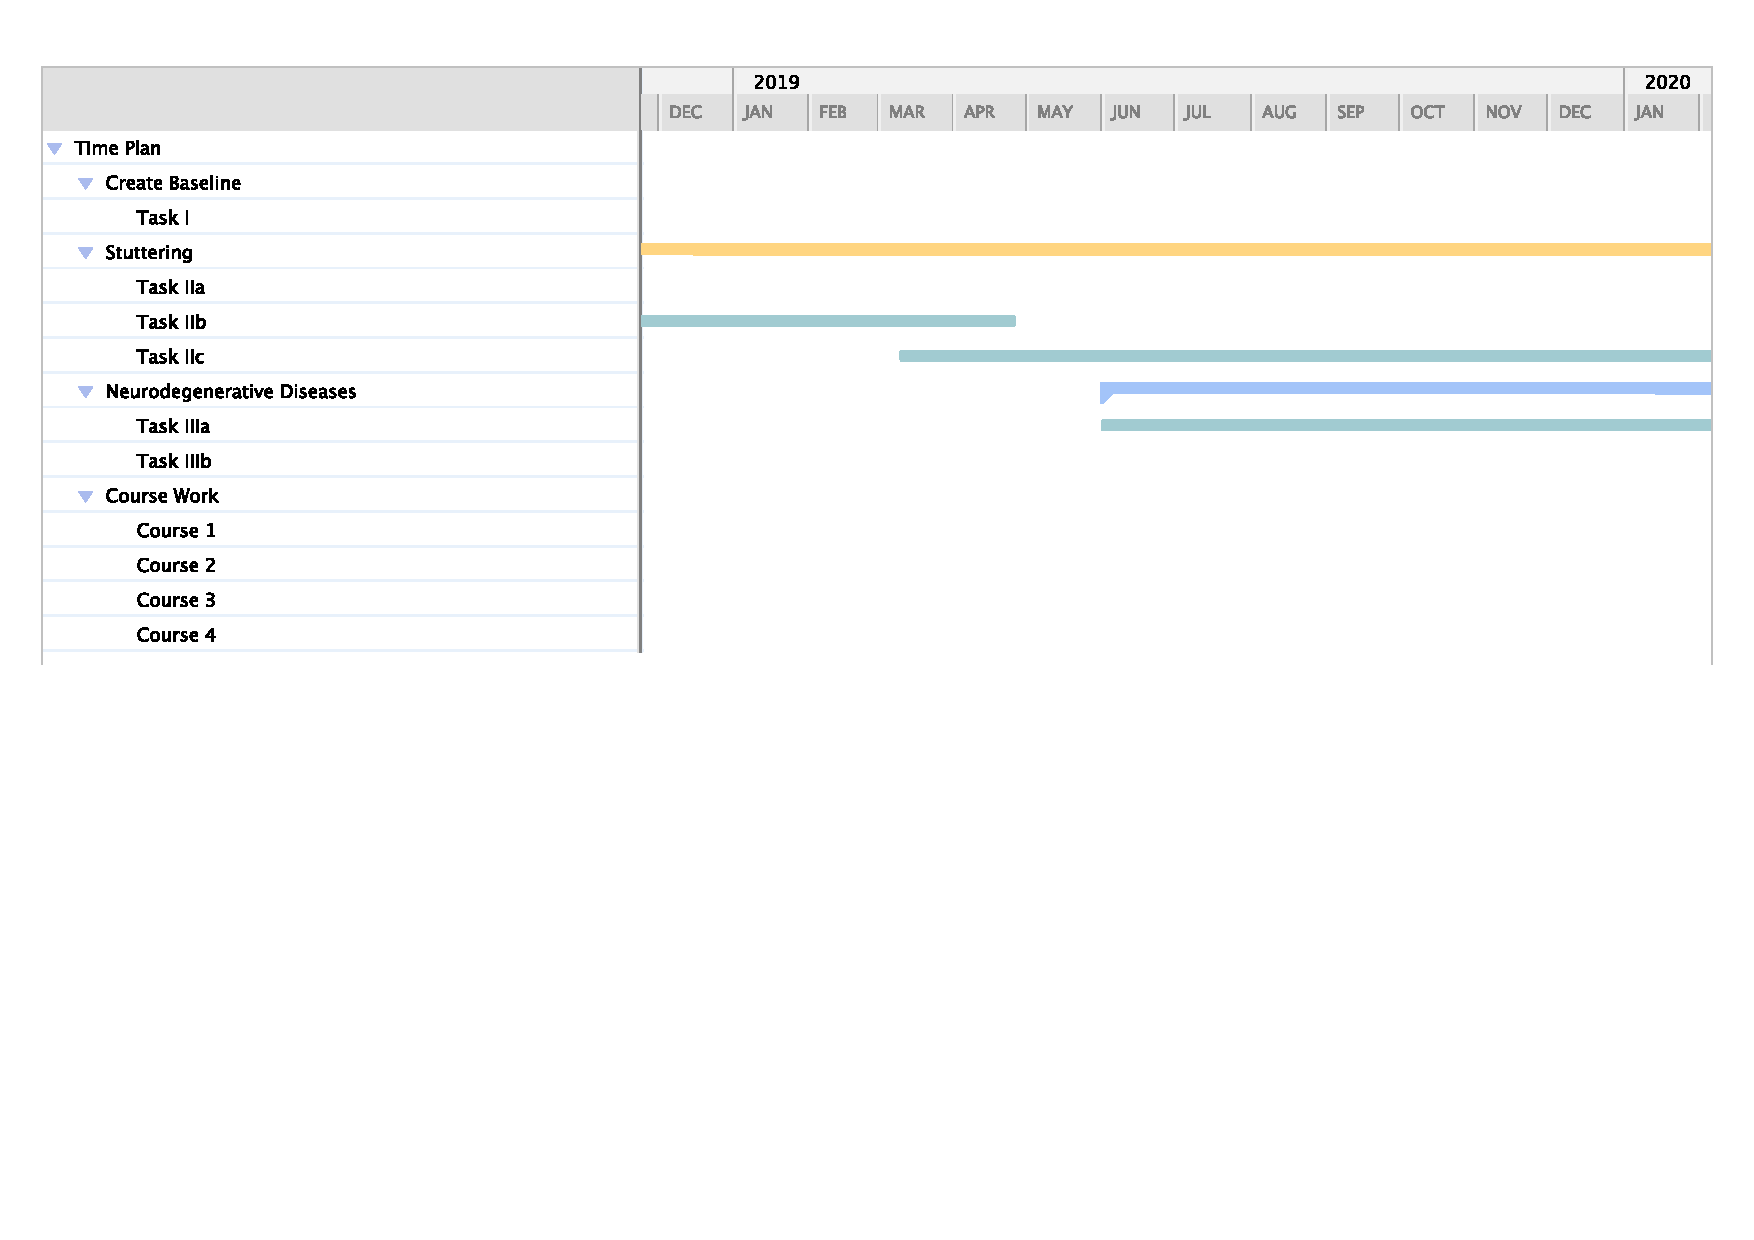
\includegraphics[width=13cm]{TimePlan3.pdf}}
\subbottom[]{
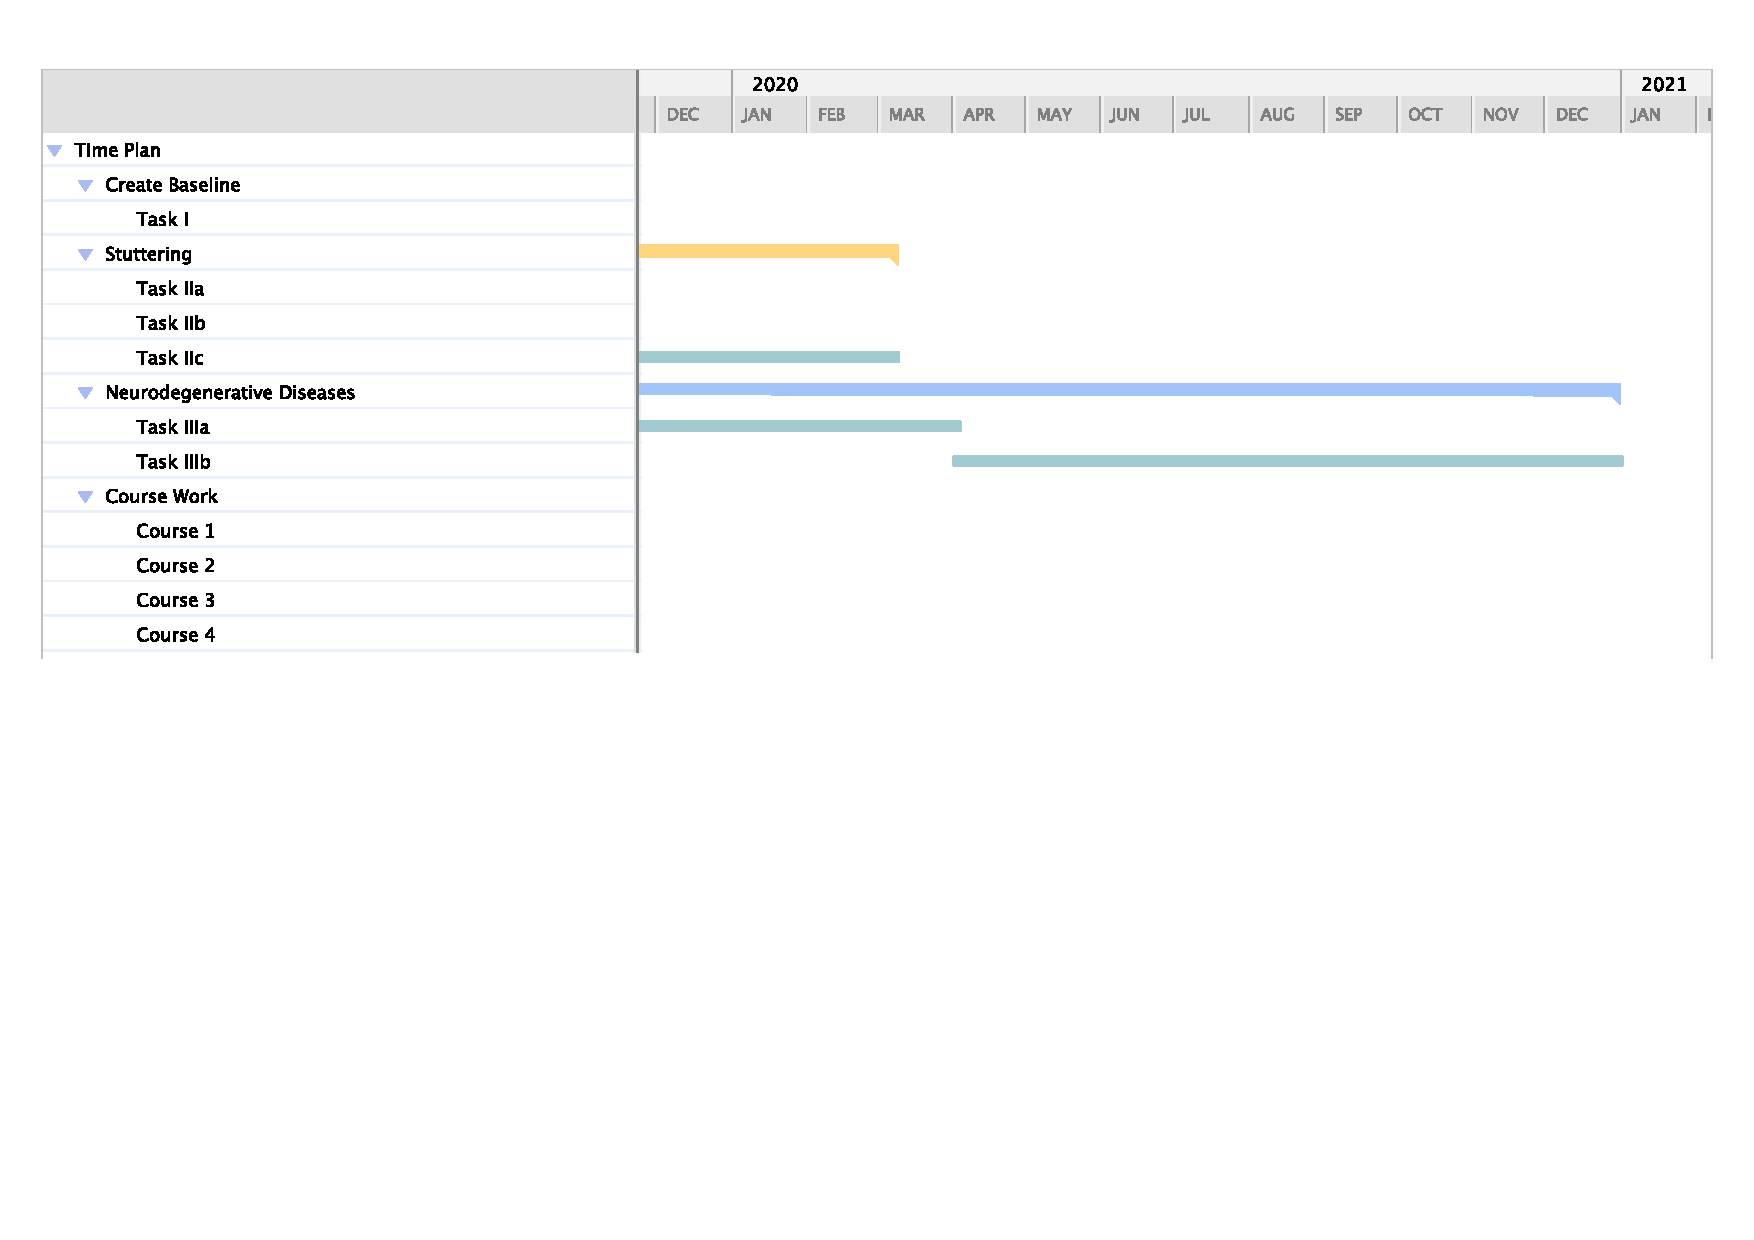
\includegraphics[width=13cm]{TimePlan4.pdf}}
\caption{Gantt chart showing the described tasks planned from August 2017 to December 2020.}
\end{figure}




\begin{comment}
\textbf{Task 1- Research image features for RGB, depth, and infrared data that permit the mapping of visible facial muscle activity to correct/incorrect execution of speech exercises OR paralysis severity.} It is expected that by combining different modalities (RGB, depth, infrared) the feature representation of facial activity is improved. The goal is that the feature representation permits the binary classification of correct/incorrect execution of speech exercises in the case of applying to speech therapy. In the case of facial paralysis the goal is to have a feature representation that permits a multiclass classification for the degree of severity of the paralysis.\\

\textbf{Task 2 - Understand the relation ... engagement during exercises through detecting relevant facial expressions.} Speech therapy requires monotonous repetition of exercises which can affect the engagement of the patient. By detecting in real-time the disengagement of the patient, different exercises can be suggested to maintain a positive learning curve. \\

\textbf{Task 3 - Research feature spaces that relates in meaningfully manner information from different modalities, therapist annotations and time.}
Suuport the SLTs reasoning and exploration of health data. 
Additionally to visual features, therapist annotations will be used to represent the progress of the therapy over time. As the therapy is performed through several sessions the time component is essential to measure the progress of a patient. 

\textbf{Task 4 - Develop statistical model that suggests future exercises by comparing one patient with similar ones in an existing database.} By being able to model the temporal progress of the therapy, the progress of one patient can be compared to the progress of others. Patients with similar starting point and positive conclusion of the therapy, can be taken as example and can provide insights of therapeutic actions that can help other similar patients to improve their progress. Thus, future actions to take can be suggested to the therapist. This model could also be used for other applications where temporal progression of a disease is observed through several therapy sessions. 


\end{comment}




